\chapter{Experimentos na camada de aplicação}

Apresentaremos os experimentos que fizemos para encontrar oportunidades de economia de energia na camada de aplicação. Após sua conclusão, o leitor verá que:

\begin{itemize}
  \item Aplicações de diferentes naturezas de utilização de recursos possuem diferentes perfis de consumo de potência.

  \item Nem sempre o algoritmo mais rápido é o que consome menos energia.

  \item Pequenas diferenças na implementação de um algoritmo podem implicar em diferenças na potência e energia consumidas.

  \item Fixados os executáveis, há um número ótimo de execuções paralelas destes programas para minimizar o consumo energético.

\end{itemize}

%\pagebreak
\section{Perfis de Consumo de Potência}
\label{power_profiles}

Queremos explorar o consumo de potência implicado pela execução de uma aplicação. Para isso, analisaremos o perfil de representantes de cada tipo de processo abaixo:

\begin{itemize}
\item \emph{CPU bound}
\item \emph{Memory bound}
\item \emph{IO bound}
\end{itemize}

Nossos três objetivos são:

\begin{itemize}
  \item Testar a granularidade de nosso sistema de medição \\
    Pode ser que nosso sistema, por sua baixa taxa de amostragem, seja muito grosseiro para detectar diferenças nos consumos de aplicações diferentes. O caso tratado por este experimento é extremo, onde as aplicações tem diferentes naturezas e, se mesmo nesse caso não conseguirmos detectar diferenças, todo o estudo ficará comprometido.

  \item Melhorar a compreensão de como uma aplicação consome potência \\
    Não encontramos nenhum material que comparasse o consumo de potência de aplicações. O mais próximo disso que encontramos foi a tese de doutoramento de Ardito \cite{ardito2014energy}, em que o autor comparou o perfil de consumo de potência de diferentes servidores.

  \item Encontrar oportunidades de melhorar a eficiência  \\energética
    Após a análise, devemos ter resultados sugerindo possibilidades de técnicas para aumentar a eficiência energética de aplicações.
\end{itemize}

Assim sendo, apesar de ser um experimento muito simples, os resultados serão utilizados nas interpretações dos próximos experimentos e no desenvolvimento de um algoritmo que troca performance por eficiência energética no segundo experimento.

\subsection{Especificação do experimento}
Para simular tarefas de diferentes naturezas, utilizamos a ferramenta de código aberto \emph{SysBench} \cite{kopytov2004sysbench}. Pode-se ver na Tabela~\ref{pow_prof_sysbench_cmd_lines} quais as linhas de comando utilizadas para os testes.

\begin{table}[h]
\centering
\begin{tabular}{|l|l|}
\hline
\emph{CPU bound}    & {\tt sysbench --test=cpu --cpu-max-prime=20000 run}                                                                                                                 \\ \hline
\emph{Memory bound} & \begin{tabular}[c]{@{}l@{}}{\tt sysbench --test=memory}\\ {\tt --memory-block-size=2G run}\end{tabular}                                             \\ \hline
\emph{IO bound}     & \begin{tabular}[c]{@{}l@{}}{\tt sysbench --test=fileio --file-total-size=24G}\\ {\tt--file-test-mode=rndrw --max-time=50}\\ {\tt --max-requests=0 run}\end{tabular} \\ \hline
\end{tabular}
\caption{Linha de comando para cada tipo de tarefa}
\label{pow_prof_sysbench_cmd_lines}
\end{table}\FloatBarrier

Também queremos observar o comportamento de cada tipo de tarefa quando executada paralelamente com outras do mesmo tipo. Assim, executamos $ i $ processos paralelos, para $ i = 1, 2, ..., 8 $, para cada tipo de tarefa.

Para cada execução, gravamos o consumo de potência e do processador através da ferramenta {\tt powerdump}. Para um determinado tipo de tarefa, utilizamos a mesma gravação para os processos paralelos fazendo intervalos de 10s a cada incremento no valor de $ i $. Pelos gráficos, o leitor não deverá encontrar dificuldades em perceber quantos processos foram utilizados.

\subsection{Resultados obtidos}

A Figura \ref{perf_pot_cpu_bound_png} mostra o consumo de potência para processos \emph{CPU Bound} rodando paralelamente.

\begin{figure}[htp]
\centering
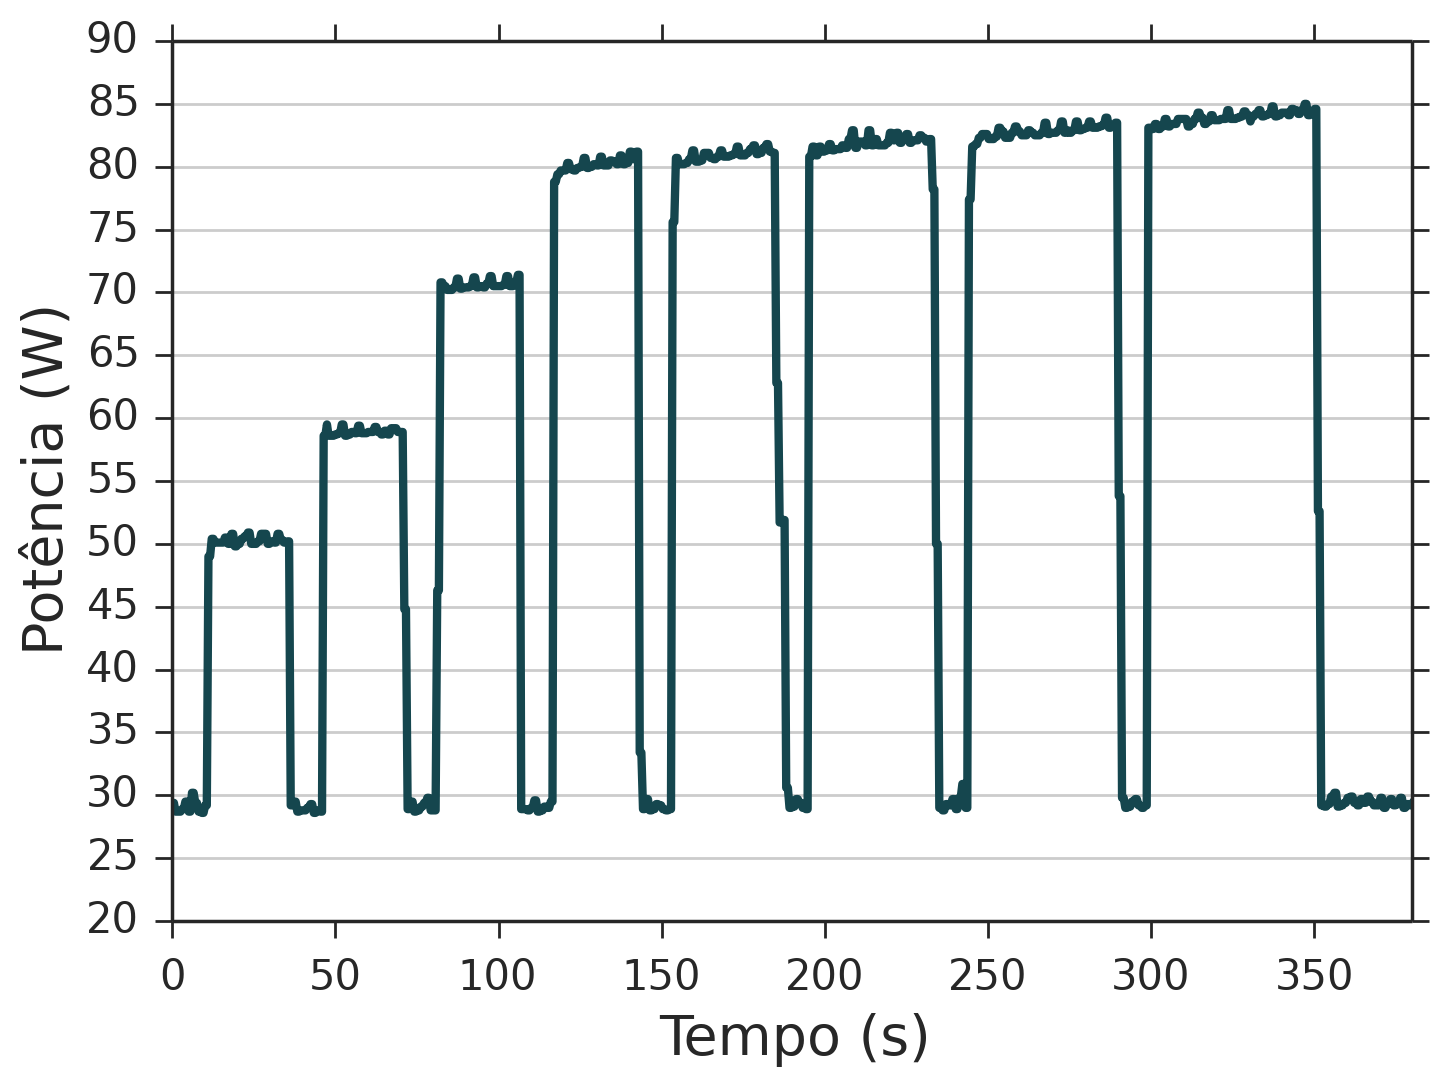
\includegraphics[scale=0.70]{figuras/Exper/PerfPot/cpubound.png}
\caption{Perfil do consumo de potência para uma tarefa \emph{CPU bound}}
\label{perf_pot_cpu_bound_png}
\end{figure}


A Figura \ref{perf_pot_mem_bound_png} mostra o consumo de potência para processos \emph{Memory Bound} rodando paralelamente.
\begin{figure}[htp]
\centering
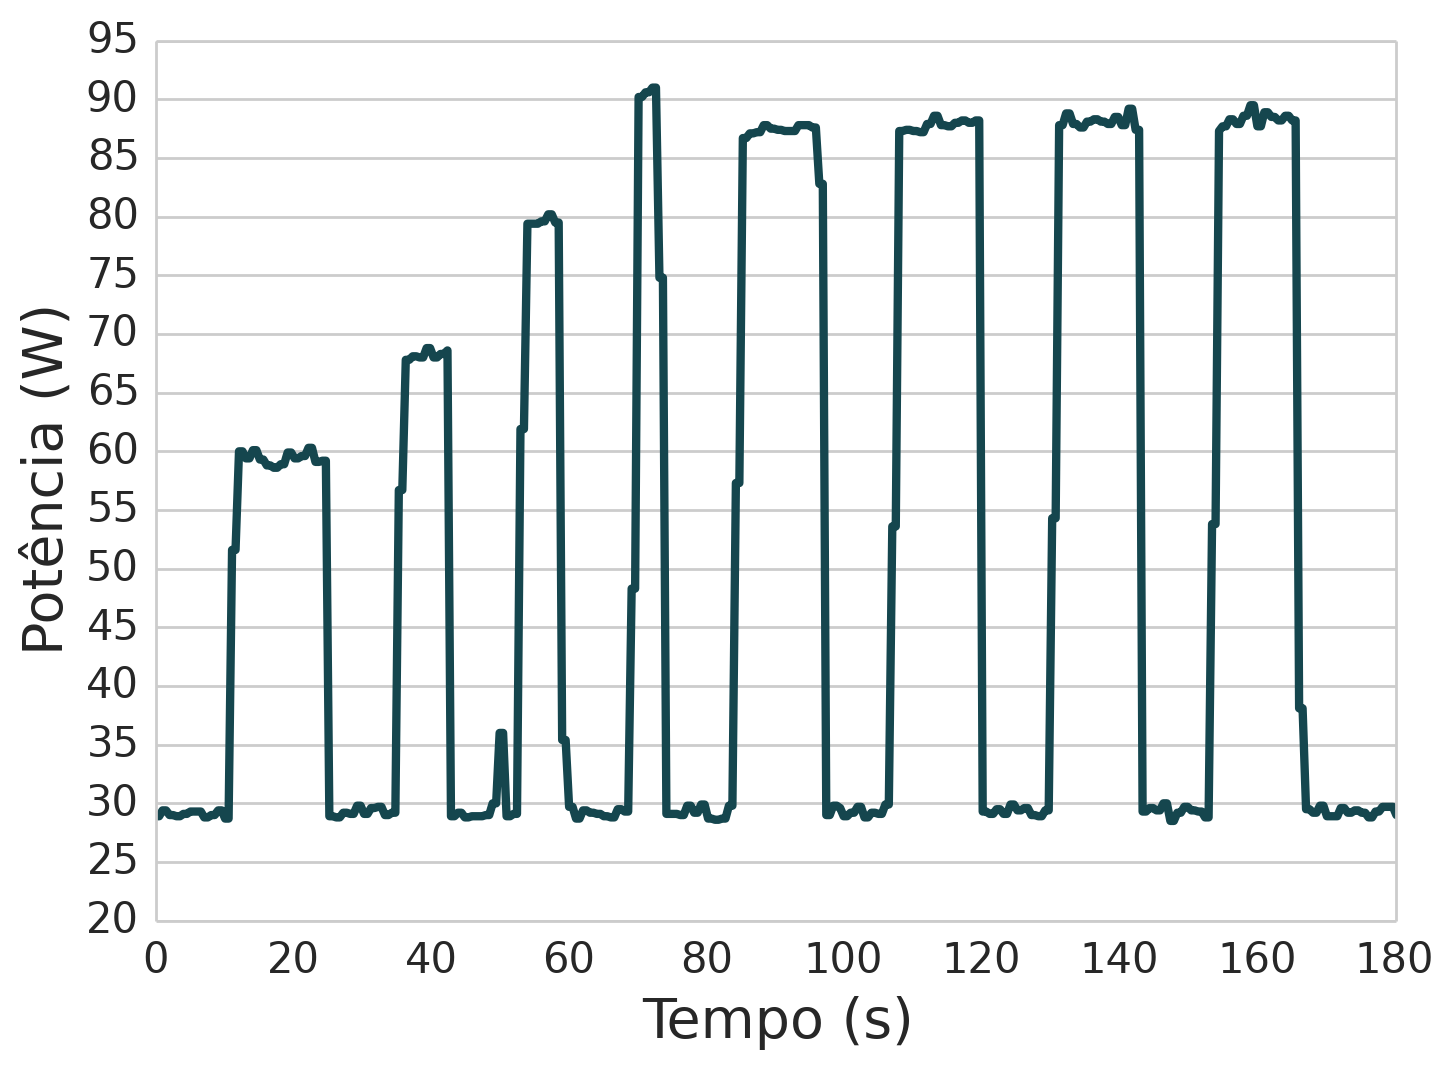
\includegraphics[scale=0.70]{figuras/Exper/PerfPot/membound.png}
\caption{Perfil do consumo de potência para uma tarefa \emph{Memory bound}}
\label{perf_pot_mem_bound_png}
\end{figure}


A Figura \ref{perf_pot_io_bound_png} mostra o consumo de potência para uma aplicação \emph{IO Bound} rodando paralelamente.
\begin{figure}[htp]
\centering
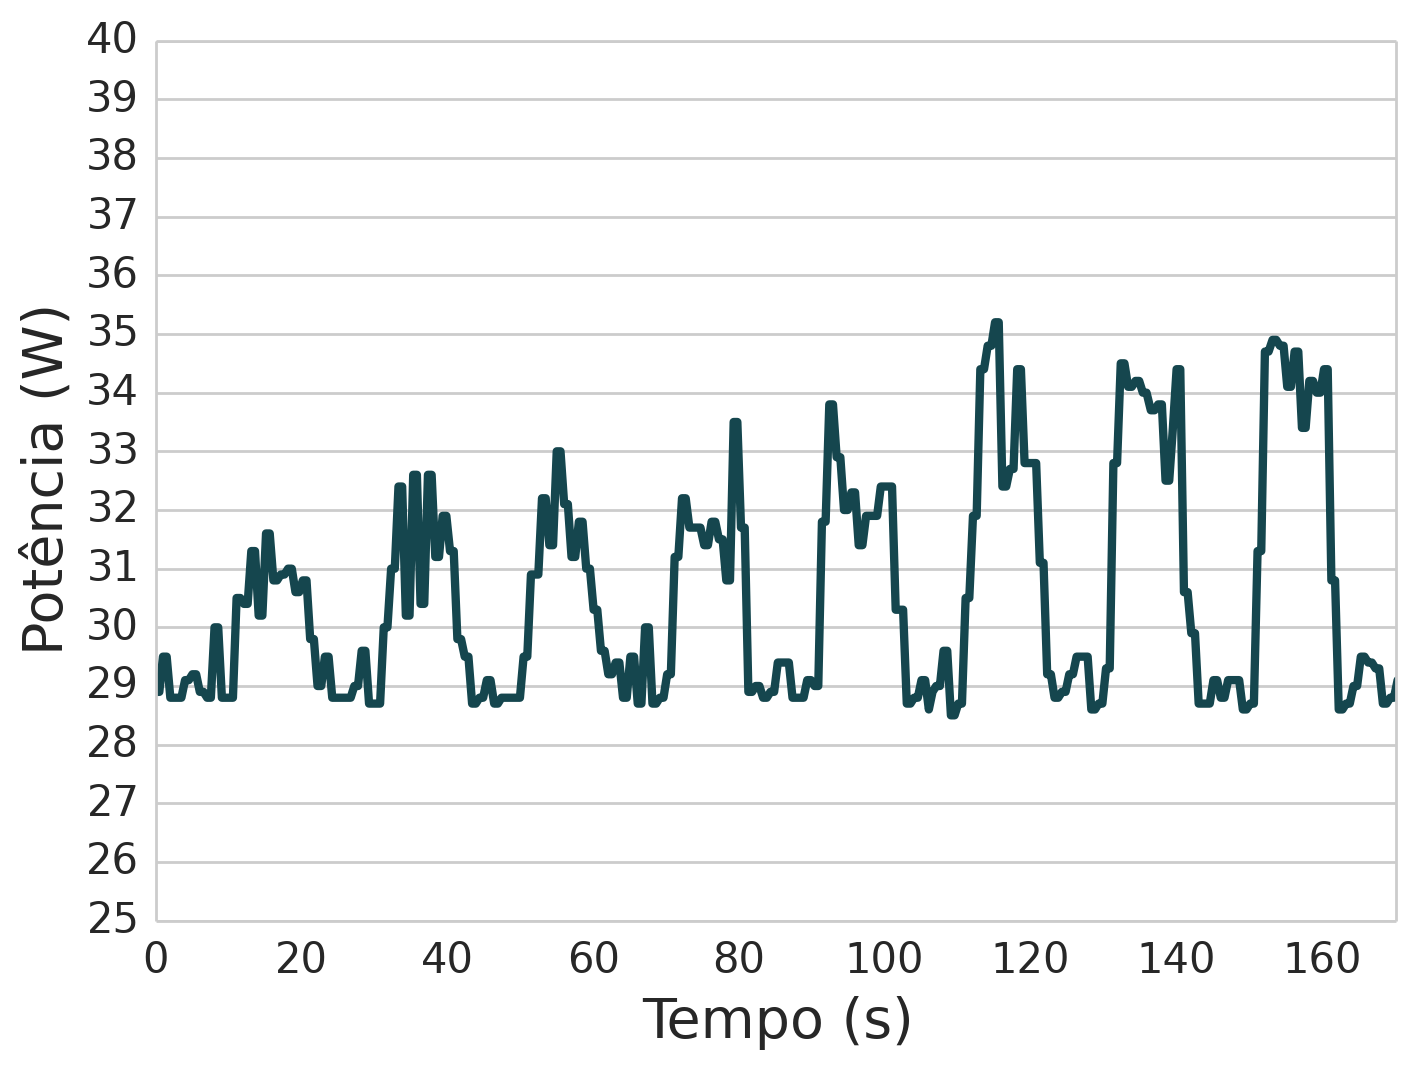
\includegraphics[scale=0.70]{figuras/Exper/PerfPot/iobound.png}
\caption{Perfil do consumo de potência para uma tarefa \emph{IO bound}}
\label{perf_pot_io_bound_png}
\end{figure}


\subsection{Análise dos resultados}

A letra $ n $ indicará o número de processos paralelos.\\

O comportamento observado dos processos \emph{CPU Bound} não é surpreendente. Até utilizarmos os quatro do processador núcleos ($ n \in \{1, 2, 3,4 \} $), não há grande diferença no tempo de execução. Nestes casos, apenas o consumo de potência cresce pois, a cada passo, passamos a usar um núcleo que estava inativo. Para $ n > 4 $, as execuções começam a demorar mais pois não há como aumentar o processamento. O que é interessante, é o aparente crescimento do consumo de potência, próximo de 5W, quando vamos de $ n = 5 $ a $ n = 8$. Este aumento no consumo parece ser de responsabilidade, provavelmente devido às trocas de contexto. Em nosso último experimento, usaremos esta observação para tentar encontrar uma oportunidade no agendamento paralelo de processos.

Sobre o comportamento dos processo \emph{Memory Bound}, vemos diretamente que os consumos são maiores que os dos processos \emph{CPU Bound}. Isso ocorre pois, neste caso temos a soma do consumo do processador com a da memória. Vemos que o comportamento observado não é tão uniforme quanto no caso \emph{CPU Bound}. O tempo de acesso à memória e a implementação do modo \emph{Memory Bound} pelo \texttt{sysbench} podem ser as causas destas diferenças. A diferença entre processos que usam a memória de modos diferentes serão exploradas nos experimentos sobre algoritmos.

Para os processos \emph{IO Bound}, vemos que é ainda menos uniforme que no caso \emph{Memory Bound}. Novamente, uma possível causa é a latência no acesso ao disco. Vemos rapidamente que o consumo é bem menor do que nos outros casos, com a maior perturbação sendo de pouco menos de 7W. Esta pequena diferença deve ser reflexo do pouco trabalho, além do que já estava considerado no consumo base do sistema, que o disco rígido faz para realizar as operações. Também há pouco uso da \emph{CPU} neste caso, que passa a maior parte do tempo em espera de operações de Entrada e Saída. \\


Com estas observações, pudemos ver que nossos sistema de medição parece ser suficiente para comparar o consumo energético de aplicações. Mostramos alguns fatores que influenciam no consumo de potência. E finalmente, conseguimos encontrar algumas oportunidades.

\section{Escolha de Algoritmos}
Esta seção é baseada no trabalho de Bunse et al. \cite{bunse2009exploring} em que os autores avaliam o desempenho energético de alguns dos algoritmos de ordenação mais comuns em dispositivos embarcados. Como estes sistemas são muito limitados, o número de entradas a serem ordenadas não passou de 1000. Sua proposta é, principalmente, responder às seguintes questões:

\begin{itemize}
  \item O consumo energético é dependente do desempenho temporal?
  \item Qual o impacto do tipo de dados no consumo energético?
\end{itemize}

Após medir o consumo energético dos algoritmos, comparam sua complexidade com o desempenho temporal, e com o consumo energético. Apesar de o tempo de execução ser bem aproximado pela complexidade, isso não ocorre para o consumo de energia. Observaram, contra nossa intuição, o \emph{insertion sort} sendo o algoritmo mais energeticamente eficiente. Segundo os autores, isso ocorre por ser o que consome menos memória.

Para examinar o impacto do tipo de dados, compararam inteiros com representações em ponto flutuante (\emph{floats}). A diferença foi muito grande, com a ordenação de \emph{floats} consumindo mais energia. Segundo os autores, isto ocorreu pois, além de \emph{floats} consumirem mais memória, os processadores dos sistemas de testes não possuíam uma \emph{Floating Point Unit}, sendo esta emulada por um software. \\

Em nosso trabalho, atacamos somente a primeira questão. Como os autores de \cite{bunse2009exploring}, comparamos algoritmos de ordenação, porém como nosso sistema é mais complexo, estamos interessados em ordenar entradas de tamanhos bem maiores. Isso faz com que no nosso caso não haja esperanças para o \emph{insertion sort}, com seu baixíssimo desempenho temporal. Assim, com base em algoritmos conhecidos, construiremos um algoritmo que consome menos potência e veremos que em alguns casos, observaremos este algoritmo consumindo menos energia mesmo perdendo em desempenho.

\subsection{Especificação do experimento}

Iremos estudar os seguintes algoritmos clássicos de ordenação:
\begin{itemize}
  \item HeapSort
  \item MergeSort
  \item QuickSort
\end{itemize}

E como candidato a algoritmo com melhor eficiência energética, usaremos uma variação esparsa do BucketSort com o InsertionSort em lista ligada sendo utilizado a cada vez que um número é adicionado a um dos \emph{buckets}. Chamaremos este algoritmo de SparseBucketSort. Escolhemos o SparseBucketSort como candidato pois tem natureza de consumo muito diferente dos outros algoritmos de ordenação.


Ainda, consideraremos 3 versões do SparseBucketSort.
\begin{itemize}
  \item $ \text{SparseBucketSort}_{0.5} $
  \item $ \text{SparseBucketSort}_{1.0} $
  \item $ \text{SparseBucketSort}_{1.5} $
\end{itemize}

Assim, se $ n $ denotar o tamanho da entrada a ser ordenada pelo algoritmo $ \text{SparseBucketSort}_{\alpha} $, o BucketSort será feito usando-se $ \alpha \times n $ \emph{buckets}.
\\

Implementamos os algoritmos em C, para ordenação de {\tt doubles}. Fizemos 30 amostras para cada algoritmo, sobre um vetor com valores uniformemente distribuídos entre 0 e {\tt RAND\_MAX}. Após a ordenação, verifica-se se o vetor foi ordenado. Os consumos para criação do vetor e verificação de corretude da ordenação não foram considerados na medição.

\subsection{Resultados obtidos}

A Figura \ref{fig:algorit_meanpower} mostra o consumo médio de potência dos algoritmos estudados.

\begin{figure}[htp]
\centering
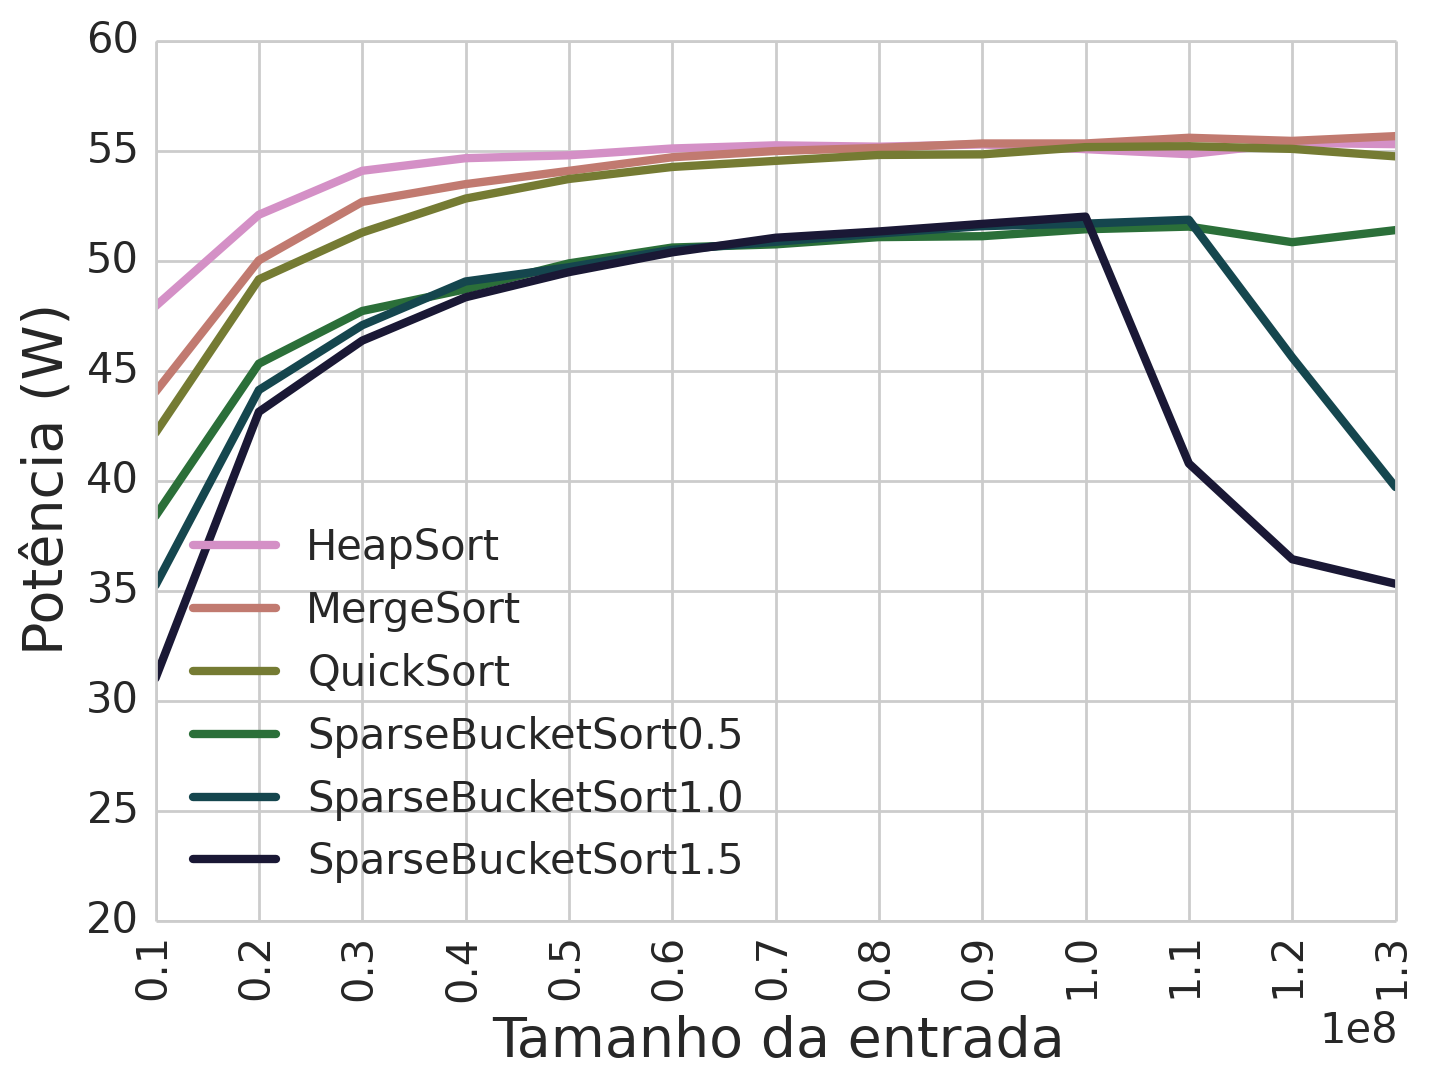
\includegraphics[scale=0.70]{figuras/Exper/Algorit/meanpower.png}
\caption{Potência consumida pelos algoritmos para diferentes tamanhos de entrada}
\label{fig:algorit_meanpower}
\end{figure}%\FloatBarrier

Na Figura \ref{fig:algorit_meantime}, pode-se ver como foi o desempenho temporal dos algoritmos.

% \begin{itemize}
%   \item $ O_{1.5} $: O $ \text{SparseBucketSort}_{1.5} $ teve o melhor desempenho temporal até esgotar a RAM. Usando o \emph{swap}, teve desempenho melhor que o HeapSort para $ n = 1.1 \times 10^8 $. Perdeu em desempenho para MergeSort com uma diferença relativa da ordem de 100\%.
%   \item $ O_{1.0} $: O $ \text{SparseBucketSort}_{1.0} $ teve o melhor desempenho temporal para $ n = 1.1 \times 10^8 $. Usando o swap, perdeu em desempenho quando $ n = 1.2 \times 10^8 $ para $ \text{SparseBucketSort}_{0.5} $, QuickSort e MergeSort.
%   \item $ O_{0.5} $: O $ \text{SparseBucketSort}_{0.5} $ perdeu em desempenho, em todos os casos observados, para o QuickSort. Chegou a ter uma diferença da ordem de 10\% no desempenho comparado ao QuickSort.
% \end{itemize}

\begin{figure}[htp]
\centering
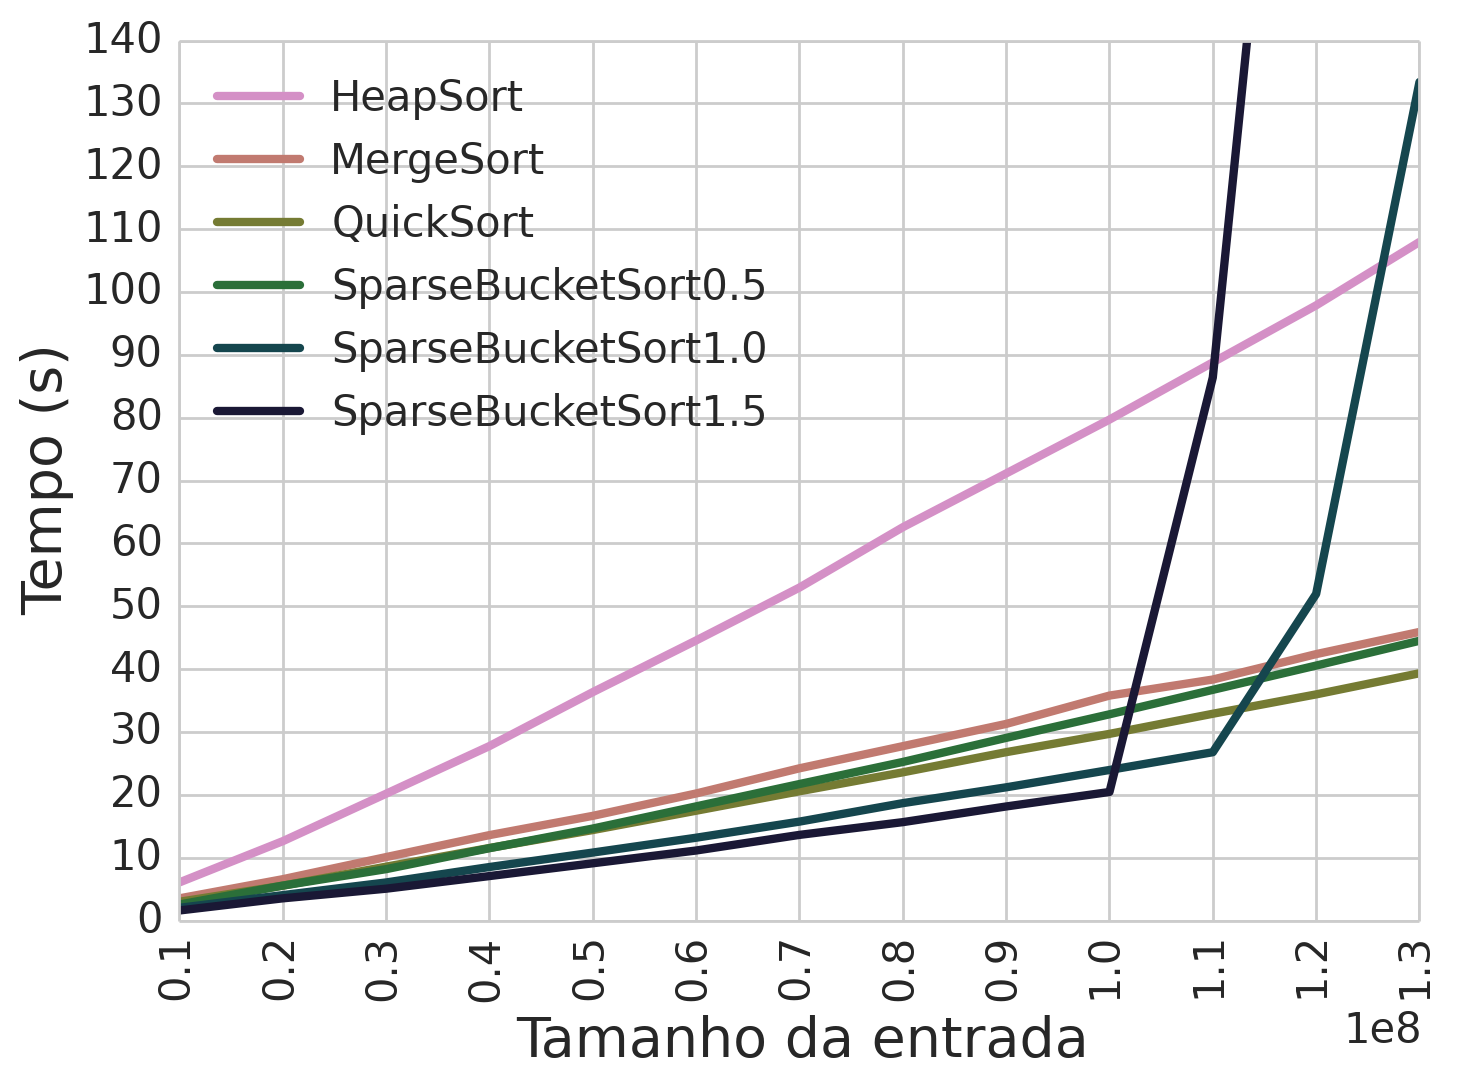
\includegraphics[scale=0.70]{figuras/Exper/Algorit/meantime.png}
\caption{Tempo de execução dos algoritmos para diferentes tamanhos de entrada}
\label{fig:algorit_meantime}
\end{figure}%\FloatBarrier

E o consumo energético de cada algoritmo pode ser visto na Figura \ref{fig:algorit_meanenergy}.

% \begin{itemize}
%   \item $ \bar{O}_{1.5} $: O $ \text{SparseBucketSort}_{1.5} $ teve consumo energético pouco melhor do que o MergeSort para $ n = 1.1 \times 10^8 $.
%   \item $ \bar{O}_{1.0} $: O $ \text{SparseBucketSort}_{1.0} $ é o que teve o menor consumo energético para $ n = 1.2 \times 10^8 $.
%   \item $ \bar{O}_{0.5} $: O $ \text{SparseBucketSort}_{0.5} $ consumiu menos energia, em todos os casos observados, que o QuickSort.
% \end{itemize}

\begin{figure}[htp]
\centering
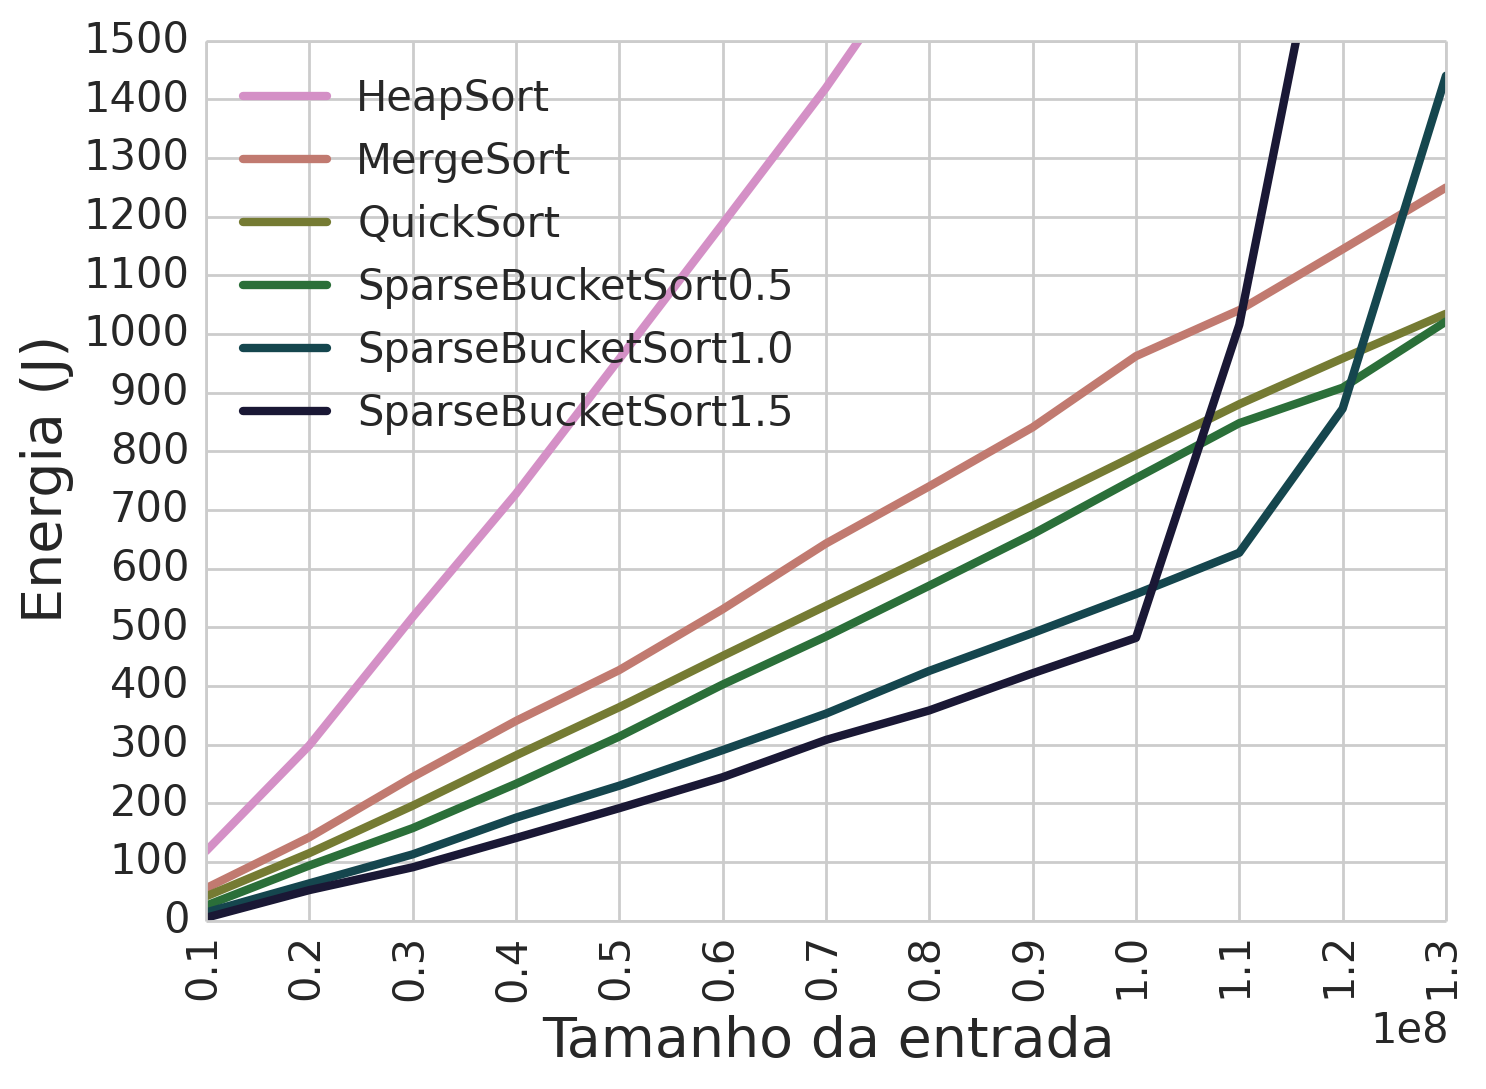
\includegraphics[scale=0.70]{figuras/Exper/Algorit/meanenergy.png}
\caption{Energia consumida pelos algoritmos para diferentes tamanhos de entrada}
\label{fig:algorit_meanenergy}
\end{figure}\FloatBarrier

\subsection{Análise dos resultados}

Primeiro, vemos pela Figura \ref{fig:algorit_meanpower} que o SparseBucketSort de fato parece consumir menos potência do que os outros. Interessante notar que o rápido decrescimento dos consumos para o $ \text{SparseBucketSort}_{1.5} $ a partir de $ n = 1.0 \times 10^8 $ e para o $ \text{SparseBucketSort}_{1.0} $ a partir de $ n = 1.1 \times 10^8 $ acontece pois estes esgotam a RAM do sistema e passam a usar o \emph{swap}. Lembrando do que foi visto sobre os perfis de consumo de potência, esse decrescimento faz sentido, pelo menor consumo de potência de aplicações \emph{CPU Bound}.

Sobre o desempenho temporal:
\begin{itemize}
  \item O $ \text{SparseBucketSort}_{1.5} $ teve o melhor desempenho temporal até esgotar a RAM. Usando o \emph{swap}, teve desempenho melhor que o HeapSort para $ n = 1.1 \times 10^8 $. Perdeu em desempenho para MergeSort com uma diferença relativa da ordem de 100\%.
  \item O $ \text{SparseBucketSort}_{1.0} $ teve o melhor desempenho temporal para $ n = 1.1 \times 10^8 $. Usando o swap, perdeu em desempenho quando $ n = 1.2 \times 10^8 $ para $ \text{SparseBucketSort}_{0.5} $, QuickSort e MergeSort.
  \item O $ \text{SparseBucketSort}_{0.5} $ perdeu em desempenho, em todos os casos observados, para o QuickSort. Chegou a ter uma diferença da ordem de 10\% no desempenho comparado ao QuickSort.
\end{itemize}

Sobre o consumo energético:
\begin{itemize}
  \item O $ \text{SparseBucketSort}_{1.5} $ teve consumo energético pouco melhor do que o MergeSort para $ n = 1.1 \times 10^8 $.
  \item O $ \text{SparseBucketSort}_{1.0} $ é o que teve o menor consumo energético para $ n = 1.2 \times 10^8 $.
  \item O $ \text{SparseBucketSort}_{0.5} $ consumiu menos energia, em todos os casos observados, que o QuickSort.
\end{itemize}

Com estas observações, mostramos que é possível construir um algoritmo com o objetivo de diminuir o consumo de potência como alternativa ao desenvolvimento baseado em performance. Porém, é importante notar que este estudo foi feito como prova de conceito, pois não nos preocupamos com uma comparação rigorosa entre os algoritmos em situações extremas nem com a escalabilidade do SparseBucketSort.

Pudemos ver claramente que nem sempre o algoritmo de melhor performance é o que consome menos energia. Isso sugere, como Bunse et al. indicaram em  \cite{bunse2009exploring}, que aplicações adaptáveis são promissores na busca por eficiência energética. Como exemplo de aplicação direta, uma aplicação que precisa ordenar uma entrada poderia escolher qual algoritmo usar dentro dos apresentados, de acordo com uma combinação entre desempenho e consumo energético passado pelo usuário.


%\pagebreak
\section{Eliminação de \emph{Code Smells}}
Esta seção é baseada no trabalho de Vetro et al. \cite{vetro2013definition}, em que os autores definem \emph{energy code smells} como padrões de código que afetam a eficiência energética de aplicações. Tentam, então, responder a duas perguntas principais:
\begin{itemize}
\item Quais \emph{code smells}\footnote{Não encontramos tradução simples e concisa. Como é bem definido em \cite{fowler1997refactoring}, deixamos no idioma original.} são \emph{energy code smells}?
\item \emph{Code smells} que impactam no consumo de energia também impactam na performance?
\end{itemize}

Para isso, os autores implementaram, em C++, funções com e sem alguns \emph{code smells} detectáveis pelos softwares \emph{CppCheck} e \emph{FindBugs}, para análise estática de código. Estes dois grupos de código foram executados num sistema embarcado, sem sistema operacional, e comparados em relação ao seu consumo energético e desempenho temporal.

Após analisar dos resultados, os autores concluíram que \emph{code smells} têm impacto, na potência média, da ordem de micro Watts e não encontraram impacto no tempo de execução. Ao final do trabalho, o ambiente de testes é apontado como principal limitação do estudo. Assim, indicam a necessidade de serem feitos estudos sobre outras plataformas. \\

Utilizando um experimento parecido, queremos validar os resultados para nosso sistema de testes, utilizando a linguagem C. Nesta seção, chamaremos de \emph{código sujo} aquele que possui um \emph{code smell}, e de \emph{código limpo}, aquele que não. As variáveis estudadas foram o tempo de execução (T), a potência média (P), e a energia consumida \textbf{pela aplicação} (E).\\

\subsection{Especificação do experimento}
Consideramos os \emph{code smells} na tabela abaixo:

\begin{table}[h]
\centering
\begin{tabular}{|l|l|}
\hline
\textit{\textbf{Code Smell}} & \textbf{Descrição}                                                                                                        \\ \hline
\emph{Dead Local Store}             & \begin{tabular}[c]{@{}l@{}}Variáveis guardam valores que não serão utilizados\\ novamente.\end{tabular} \\ \hline
\emph{Non Short Circuit}            & \begin{tabular}[c]{@{}l@{}}Operador lógico na expressão não é de curto\\ circuito.\end{tabular}                           \\ \hline
Parameter By Value           & \begin{tabular}[c]{@{}l@{}}Parâmetro de função passado por valor, não \\ referência.\end{tabular}                         \\ \hline
\emph{Redundant Function Call}      & \begin{tabular}[c]{@{}l@{}}Chamada de função sobre os mesmo parâmetros \\ a cada iteração.\end{tabular}                   \\ \hline
\emph{Repeated Conditional}         & \begin{tabular}[c]{@{}l@{}}Bloco condicional dentro de outro sobre mesma \\ expressão.\end{tabular}                       \\ \hline
\emph{Self Assignement}             & \begin{tabular}[c]{@{}l@{}}Atribuição do valor de uma variável à ela mesma. \\ \end{tabular}                       \\ \hline
\end{tabular}
\caption{\emph{Code smells} considerados}
\end{table}\FloatBarrier

Dentre eles, apenas o \emph{Redundant Function Call} não foi considerado pelos autores de \cite{vetro2013definition}. Além disso, todos os outros são aqueles indicados no artigo como \emph{energy code smells}. \\

Chamamos limpo, o código sem \emph{code smells} e sujo, aquele com o respectivo \emph{code smell}. Escrevemos código limpo e sujo para cada padrão. Todos os códigos foram compilados utilizando o gcc (v.4.6.3) sem otimizações para evitar que o próprio compilador fizesse a eliminação e não pudéssemos identificar seu impacto.

Abaixo, um exemplo para o \emph{code smell} \emph{Non Short Circuit}. Temos o código com o \emph{code smell} à esquerda, e depois de sua eliminação, à direita.

\begin{center}
\begin{minipage}{.48\textwidth}
\begin{lstlisting}[language=C, basicstyle=\scriptsize\ttfamily, frame=single]
#include <stdlib.h>

void non_short_circuit();

int main(int argc, char *argv[]) {
    long i, n;

    n = atoi(argv[1]);
    for (i = 0; i < n; i++)
        non_short_circuit();
    return 0;
}

void non_short_circuit() {
    int a, b;

    a = rand();
    b = rand();
    if ((a < b) & (b > a)) {
        a += b;
        return;
    }
    b += a;
}
\end{lstlisting}
\end{minipage}
\hfill
\begin{minipage}{.48\textwidth}
\begin{lstlisting}[language=C, basicstyle=\scriptsize\ttfamily, frame=single]
#include <stdlib.h>

void wo_non_short_circuit();

int main(int argc, char *argv[]) {
    long i, n;

    n = atoi(argv[1]);
    for (i = 0; i < n; i++)
        wo_non_short_circuit();
    return 0;
}

void wo_non_short_circuit() {
    int a, b;

    a = rand();
    b = rand();
    if ((a < b) && (b > a)) {
        a += b;
        return;
    }
    b += a;
}
\end{lstlisting}
\end{minipage}
\end{center}


Como chamadas de funções podem ser muito rápidas, para fazer medições sobre o consumo de funções é necessário fazer várias iterações sobre suas chamadas a cada execução do programa. Para isso, os \emph{code smells} foram implementados em funções e o número de chamadas dessas funções é dado pelo argumento passado em linha de comando na execução do programa. Este número é diferente para cada padrão testado, dependente do tempo de execução da função. Embora, evidentemente, seja o mesmo número para as versões limpas e sujas de um mesmo código.

Com $ n = 50 $ medições através do {\tt energyanalyser}, conseguimos os resultados apresentados na próxima seção.

%\pagebreak
\subsection{Resultados obtidos}
 Tabela \ref{tab:cs_medias_variaveis} contém os valores das médias amostrais de cada variável estudada. Nesta seção T indica o tempo, P a potência média\footnote{Assim, $ \bar{P} $ indicará a médias das potências médias observadas.} e E a energia consumida, medidas em segundos, Watts e Joules, respectivamente. Os índices S e L indicam as medições sobre, respectivamente, os códigos sujos e limpos.

\begin{table}[h]
\centering
\begin{tabular}{l|l|l|l|l|l|l|}
\cline{2-7}
                                            & \multicolumn{3}{c|}{\textbf{Sujo}}                   & \multicolumn{3}{c|}{\textbf{Limpo}}                  \\ \hline
\multicolumn{1}{|l|}{\textit{Code Smell}}   & $ \bar{T}_{S} $ (s) & $ \bar{P}_{S} $ (W) & $ \bar{E}_{S} $  (J) & $ \bar{T}_{L} $  (s) & $ \bar{P}_{L} $ (W) & $ \bar{E}_{L} $ (J) \\ \hline
\multicolumn{1}{|l|}{Dead Local Store}      & 7.7319          & 50.2840         & 155.8870         & 5.3567           & 50.0569         & 104.8748        \\ \hline
\multicolumn{1}{|l|}{Non Short Circuit}     & 9.8608          & 52.7283         & 222.2495         & 9.7011           & 52.3865         & 214.3383        \\ \hline
\multicolumn{1}{|l|}{Redundant Call}        & 8.7104          & 52.3006         & 190.6049         & 3.9796           & 45.2733         & 59.6092         \\ \hline
\multicolumn{1}{|l|}{Repeated Conditionals} & 9.8446          & 52.7815         & 219.2489         & 9.4782           & 52.5596         & 213.5707        \\ \hline
\multicolumn{1}{|l|}{Parameter by Value}    & 11.1594         & 53.4761         & 257.4827         & 8.5002           & 52.6891         & 190.6035        \\ \hline
\multicolumn{1}{|l|}{Self Assignement}      & 9.5107          & 53.5184         & 218.6024         & 9.5105           & 52.9153         & 215.0994        \\ \hline
\end{tabular}
\caption{Médias amostrais das variáveis estudadas}
\label{tab:cs_medias_variaveis}
\end{table}
\FloatBarrier

A Figura \ref{fig:cs_barplot_all} mostra o impacto, em cada variável, da eliminação de cada \emph{code smell}.

\begin{figure}[htp]
\centering
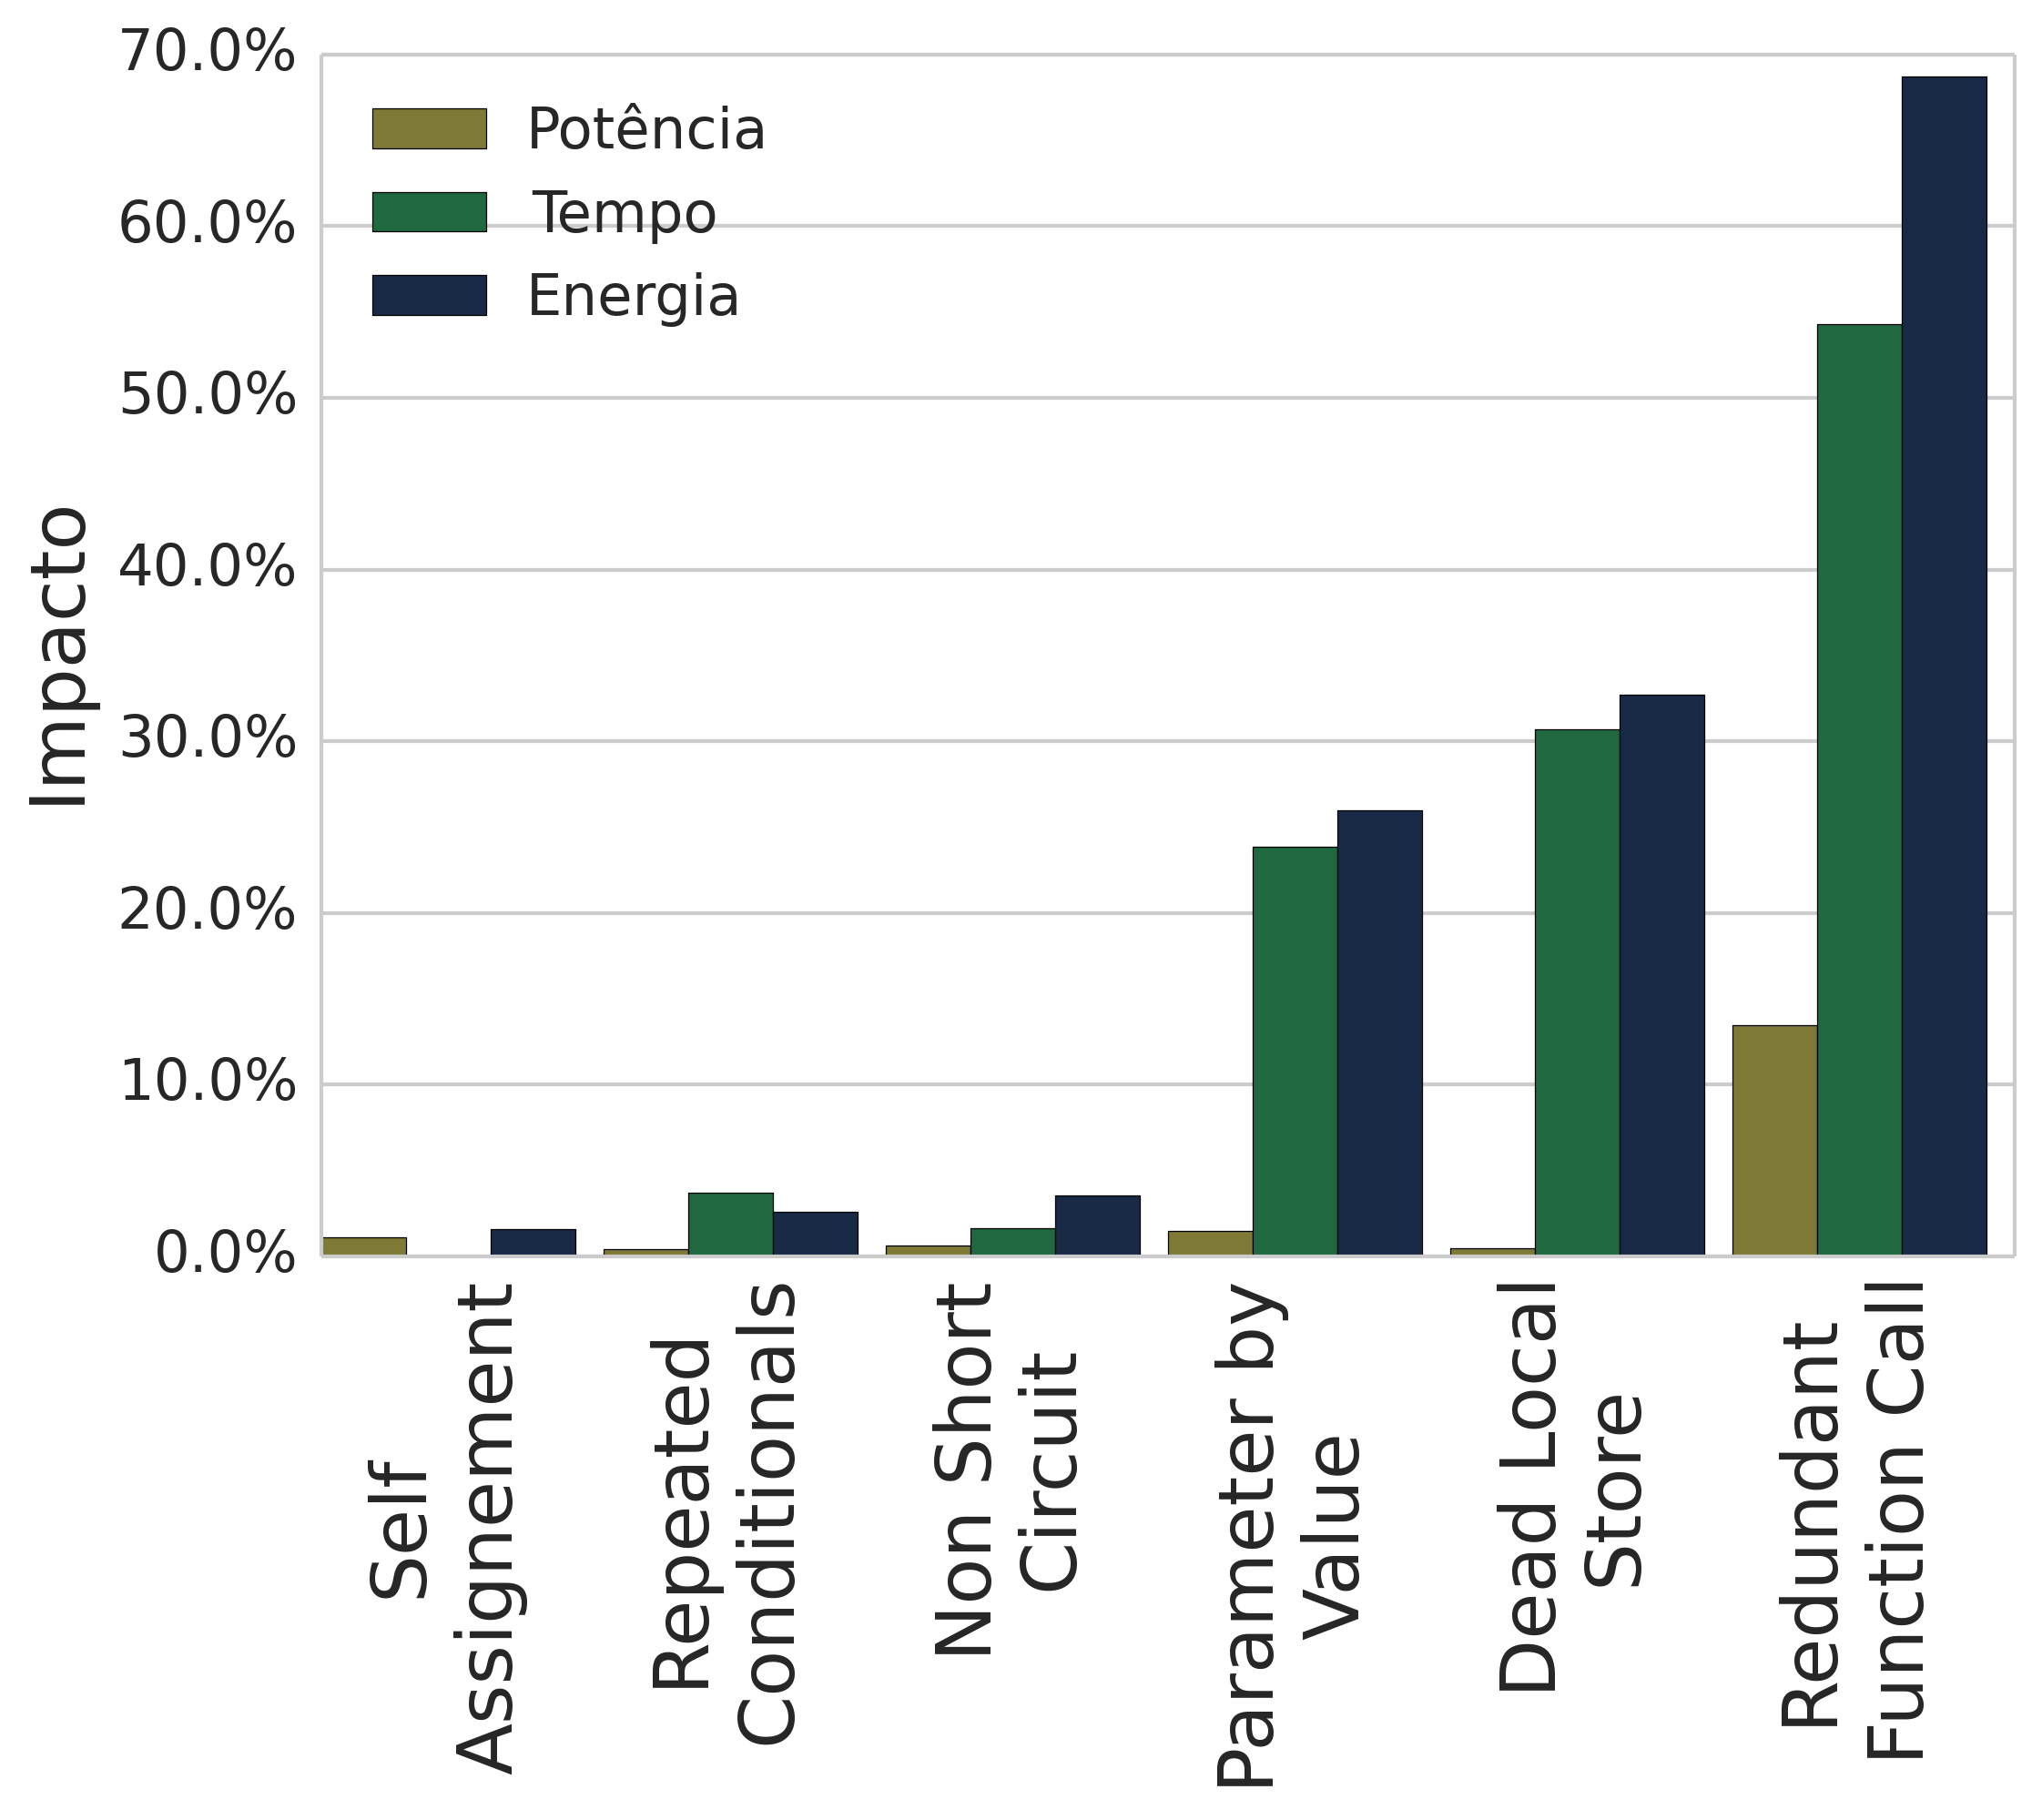
\includegraphics[scale=0.70]{figuras/Exper/CodeSmells/codesmells_impact.png}
\caption{Impacto médio da retirada de cada \emph{code smell} nas variáveis de interesse}
\label{fig:cs_barplot_all}
\end{figure}\FloatBarrier

Ainda, a Tabela \ref{tab:cs_impact} contém os cálculos dos impactos apresentados na Figura \ref{fig:cs_barplot_all}.

\begin{table}[h]
\centering
\begin{tabular}{|l|l|l|l|}
\hline
\textit{Code Smell}            & $ \frac{\bar{T}_{S} - \bar{T}_{L}}{\bar{T}_{S}} $ & $ \frac{\bar{P}_{S} - \bar{P}_{L}}{\bar{P}_{S}} $ & $ \frac{\bar{E}_{S} - \bar{E}_{L}}{\bar{E}_{S}} $ \\ \hline
\textit{Dead Local Store}      & 30.72\%                                           & 0.45\%                                            & 32.72\%                                           \\ \hline
\textit{Non Short Circuit}     & 1.62\%                                            & 0.65\%                                            & 3.56\%                                            \\ \hline
\textit{Redundant Call}        & 54.31\%                                           & 13.44\%                                           & 68.73\%                                           \\ \hline
\textit{Repeated Conditionals} & 3.72\%                                            & 0.42\%                                            & 2.59\%                                            \\ \hline
\textit{Parameter by Value}    & 23.83\%                                           & 1.47\%                                            & 25.97\%                                           \\ \hline
\textit{Self Assignement}      & 0.00\%                                            & 1.13\%                                            & 1.60\%                                            \\ \hline
\end{tabular}
\caption{Tabela de impacto da eliminação de cada \emph{code smell}}
\label{tab:cs_impact}
\end{table}

\subsection{Análise dos resultados}
Pela Tabela \ref{tab:cs_impact}, podemos ver que, exceto pelos padrões \emph{Redundant Call} e \emph{Self Assignement}, a diferença no tempo de execução parece ser a principal causa da diminuição do consumo energético. Este se opõe ao que foi encontrado pelos autores de \cite{vetro2013definition}.

Também diferente do encontrado em \cite{vetro2013definition}, a diferença de potência encontrada foi, pelo menos, da ordem de, pelo menos, $ 10^{-3} $ Watts, não $ 10^{-6} $, como o artigo mostra. Porém esta diferença era esperada pois o sistema embarcado utilizado em \cite{vetro2013definition} tinha um nível de consumo muito menor.

Além das diferenças apresentadas entre as duas configurações, uma das possíveis causas destas diferenças é o pequeno número de repetições das funções que os autores do artigo utilizaram, de 1.000.000, enquanto nossos números de repetição vão de 40.000.000 a 1.000.000.000. \\\\

De qualquer forma, o impacto de \emph{code smells} na eficiência energética de uma aplicação é da ordem de nJ, que é quase imperceptível. Assim, o estudo da eliminação de \emph{code smells} a fim de economizar energia não parece ser muito promissor, porém pode melhorar o entendimento de como uma aplicação pode gastar energia.

Estas diferenças de resultados também mostram que os resultados sobre eficiência energética encontrados para dispositivos móveis ou embarcados podem não valer para computadores pessoais e servidores. Novamente, a validação de resultados para diferentes plataformas é justificada.

%\pagebreak
\section{Agendamento de Processos}
Nesta seção, estudaremos como o escalonamento de processos pode impactar na eficiência energética de nosso sistema. Em particular, queremos saber como, para uma certa tarefa dada por vários processos, a escolha do número máximo de processos paralelos impacta no consumo de energia.

Importante lembrar que, teoricamente, o agendamento de processos é serviço do sistema operacional. Porém, como nossos privilégios são limitados na máquina de testes, este estudo foi feito na camada de aplicação.

\subsection{Especificação do experimento}
Consideramos, como tarefa, a execução de 32 processos do programa {\tt pidigits 30000}. A aplicação {\tt pidigits} faz parte do projeto \emph{The Computer Language Benchmarks Game} \cite{benchgame}. Para mostrar que o agendamento de processos impacta na eficiência energética, usaremos o {\tt energyanalyser} com 50 observações para cada $ n = 1, 2, ..., 32 $, sobre o procedimento descrito abaixo:

\begin{itemize}

\item Execute os 32 processos, porém permitindo que no máximo $ n $ processos rodem paralelamente.

\end{itemize}
Realizamos este procedimento com a ferramenta GNU Parallel \cite{tange2011gnu}. \\

Com isso, esperamos encontrar diferenças significativas no consumo energético para cada valor de $ n $. Ainda, se isto ocorrer, tentaremos encontrar um $ n $ ótimo, que minimize o consumo energético total.

\subsection{Resultados obtidos}
Primeiramente, pode-se ver como a potência varia em função de $ n $ na Figura \ref{fig:agendamento_meanpower}.

\begin{figure}[htp]
\centering
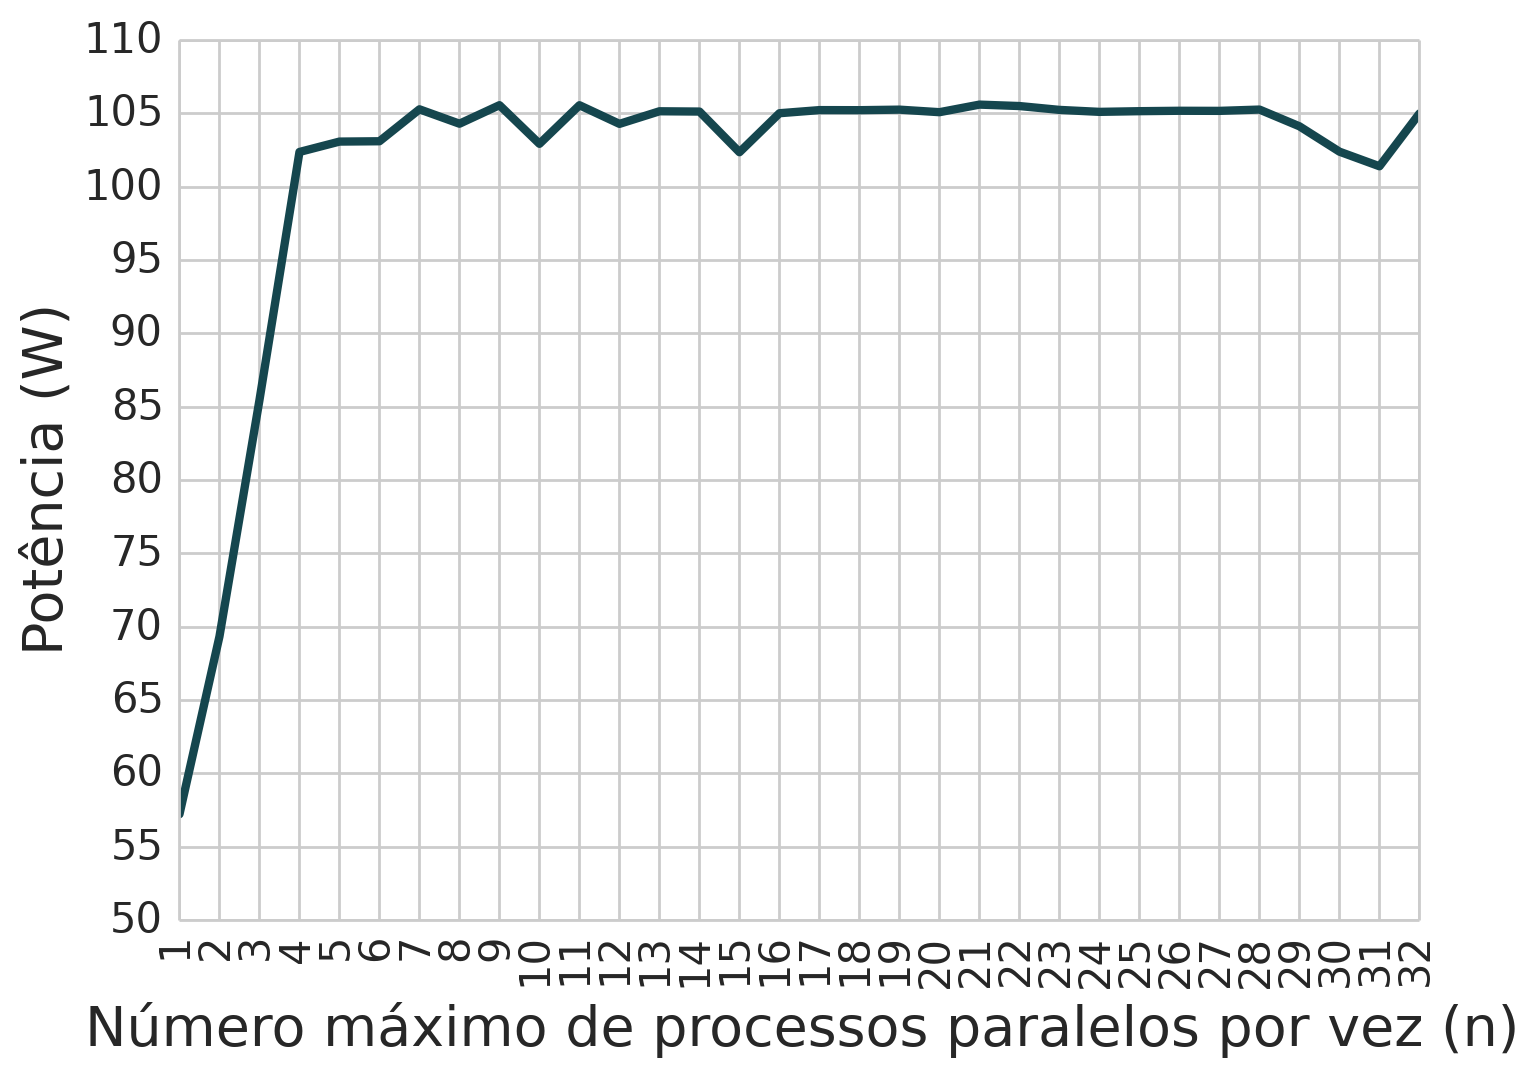
\includegraphics[scale=0.70]{figuras/Exper/AgendProc/meanpower.png}
\caption{Potência média consumida pelo sistema para cada $ n $ }
\label{fig:agendamento_meanpower}
\end{figure}

A Figura \ref{fig:agendamento_meantime} mostra que o $ n $ ótimo para performance observado foi de $ n = 7 $.

\begin{figure}[htp]
\centering
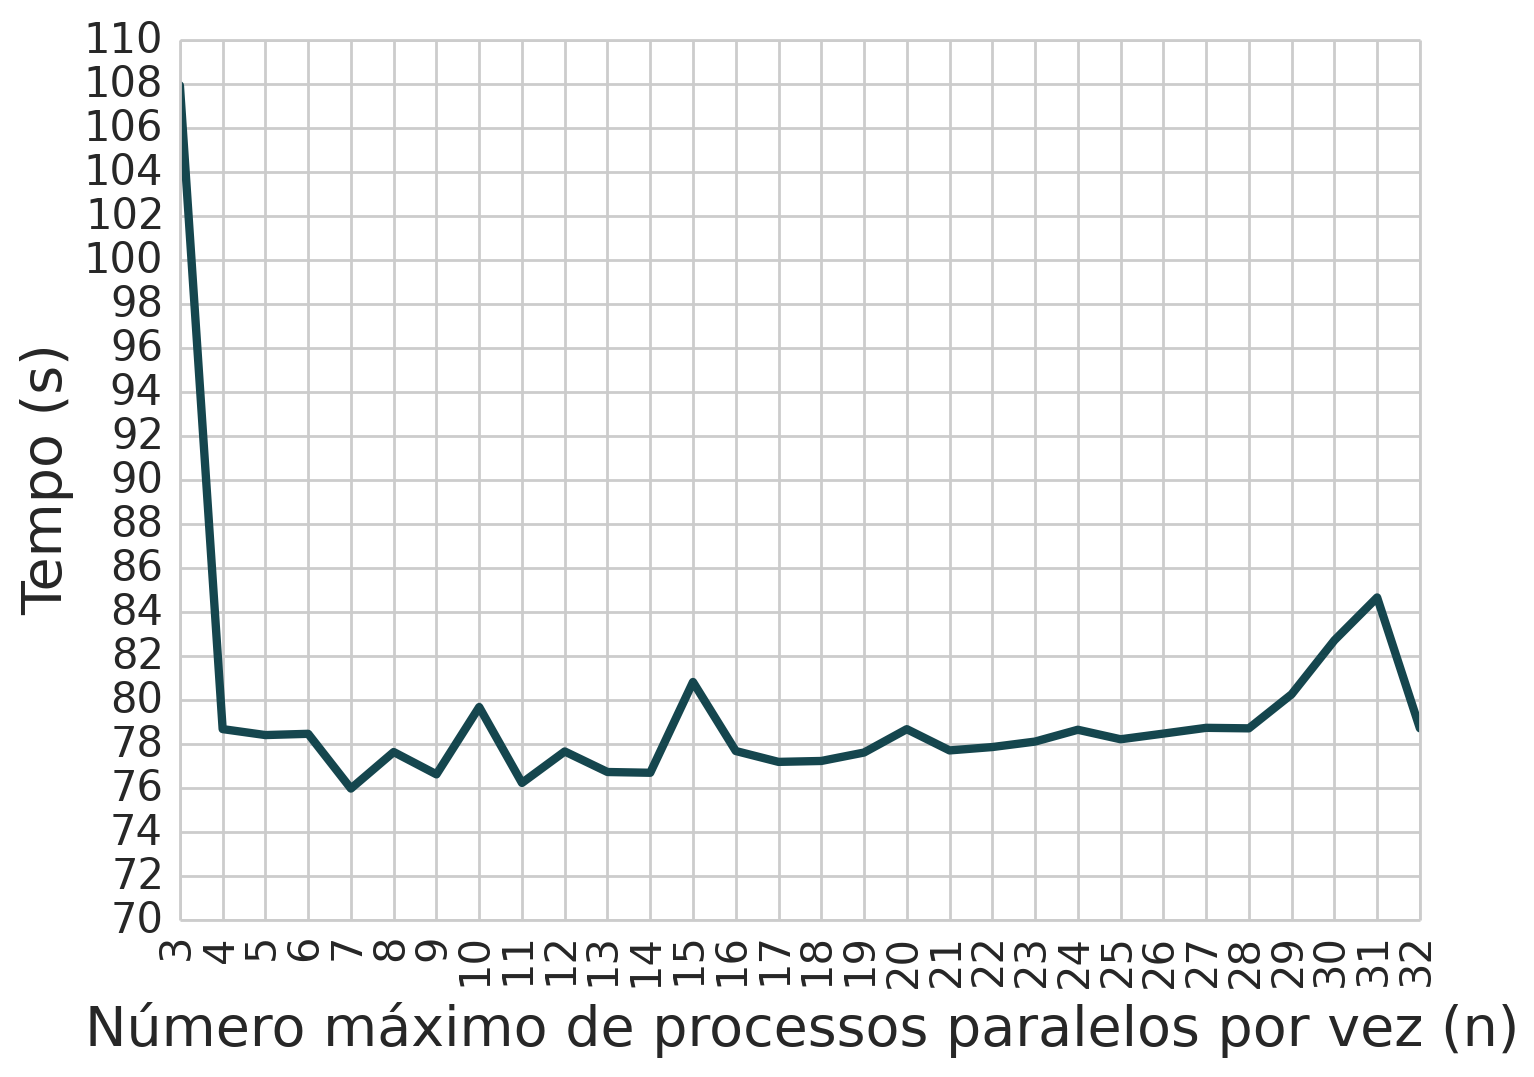
\includegraphics[scale=0.70]{figuras/Exper/AgendProc/meantime.png}
\caption{Tempo médio de execução da tarefa para cada $ n $ }
\label{fig:agendamento_meantime}
\end{figure}

O consumo energético descontando o consumo do sistema pode ser visto na Figura \ref{fig:agendamento_meanenergy}. Este gráfico sugere que $ n = 4 $ é ótimo para energia. Porém, como trata-se de um agendamento, o objetivo é minimizar o consumo de todo o sistema. Este consumo total é mostrado na Figura \ref{fig:agendamento_totenergy}. Neste caso, o $ n $ ótimo observado foi $ n = 7 $.

\begin{figure}[htp]
\centering
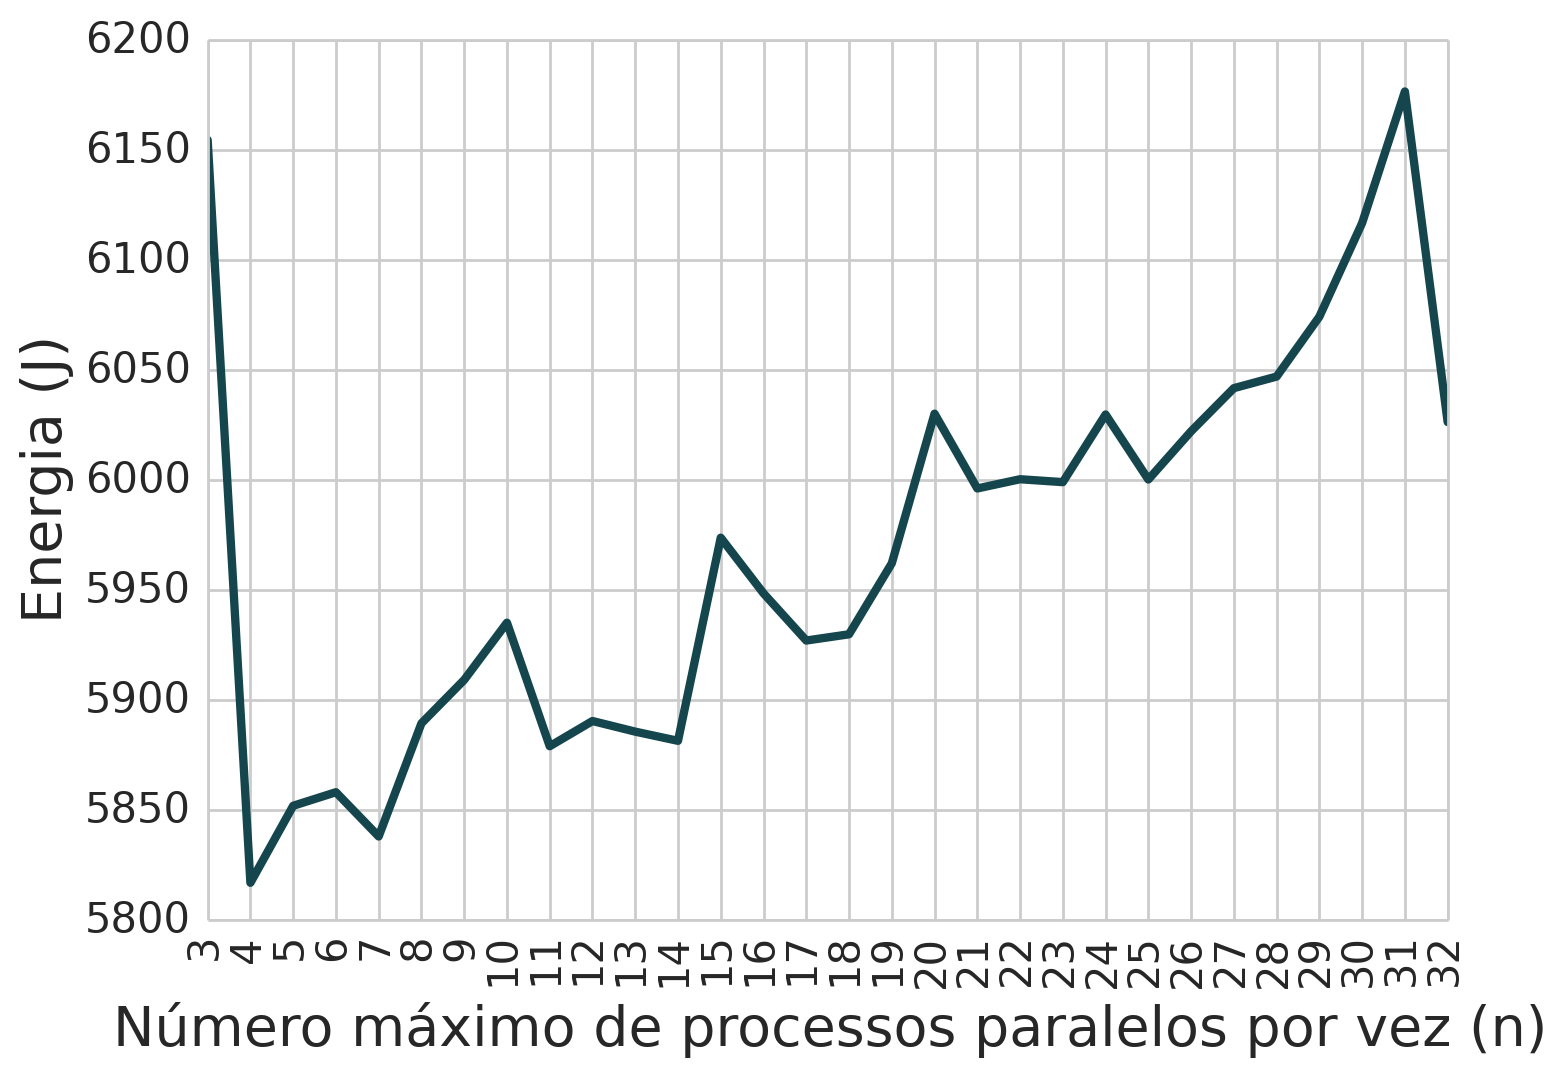
\includegraphics[scale=0.70]{figuras/Exper/AgendProc/meanenergy.png}
\caption{Energia média consumida pela tarefa para cada $ n $ }
\label{fig:agendamento_meanenergy}
\end{figure}

\begin{figure}[htp]
\centering
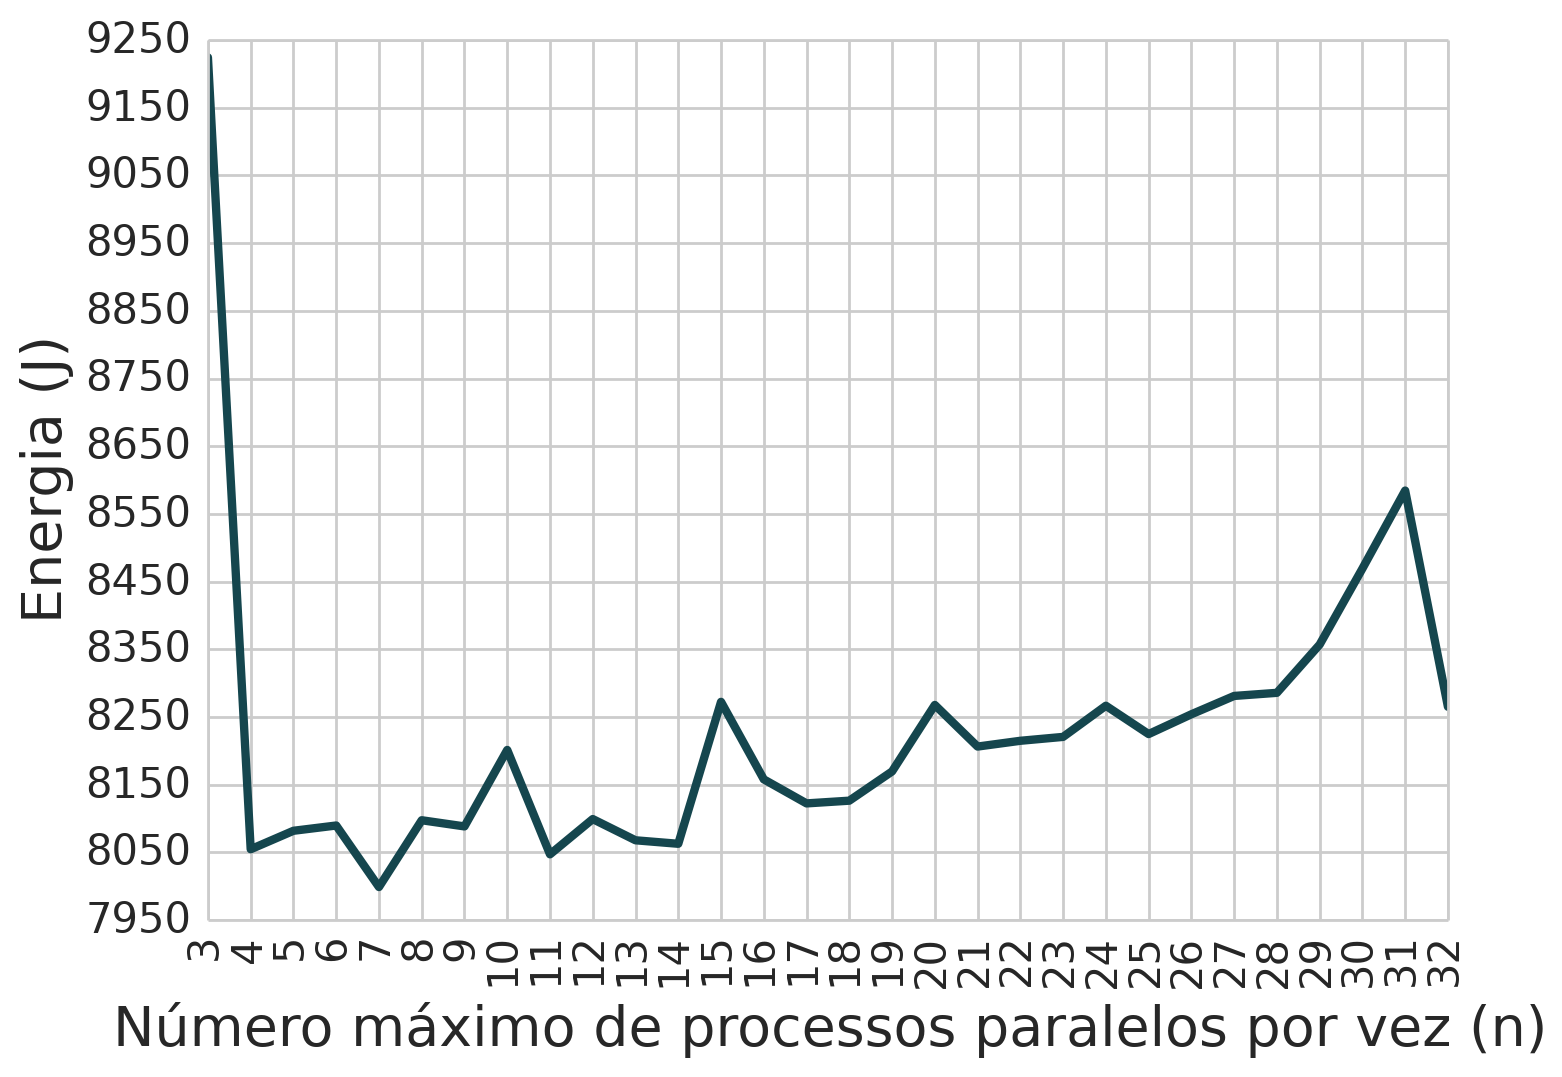
\includegraphics[scale=0.70]{figuras/Exper/AgendProc/meantotenergy.png}
\caption{Energia média consumida pelo sistema para cada $ n $ }
\label{fig:agendamento_totenergy}
\end{figure}


Seja $ \bar{E}(i) $ o consumo energético total utilizando $ n = i $, a Tabela~\ref{agend_proc_energy_impact} mostra a melhora pela utilização de $ n = 7 $.

\begin{table}[h]
\centering
\begin{tabular}{ll|ll|ll|ll}
$ n $ & \textbf{$ \frac{\bar{E}(n) - \bar{E}(7)}{\bar{E}(7)} $} & $ n $ & \textbf{$ \frac{\bar{E}(n) - \bar{E}(7)}{\bar{E}(7)} $} & $ n $ & \textbf{$ \frac{\bar{E}(n) - \bar{E}(7)}{\bar{E}(7)} $} & $ n $ & \textbf{$ \frac{\bar{E}(n) - \bar{E}(7)}{\bar{E}(7)} $} \\ \hline
1     & 103.51\%         & 9     & 1.12\%           & 17    & 1.54\%           & 25    & 2.82\%           \\
2     & 35.59\%          & 10    & 2.53\%           & 18    & 1.59\%           & 26    & 3.19\%           \\
3     & 15.32\%          & 11    & 0.60\%           & 19    & 2.13\%           & 27    & 3.53\%           \\
4     & 0.70\%           & 12    & 1.26\%           & 20    & 3.36\%           & 28    & 3.59\%           \\
5     & 1.04\%           & 13    & 0.86\%           & 21    & 2.59\%           & 29    & 4.48\%           \\
6     & 1.14\%           & 14    & 0.80\%           & 22    & 2.70\%           & 30    & 5.88\%           \\
7     & 0.00\%           & 15    & 3.42\%           & 23    & 2.77\%           & 31    & 7.32\%           \\
8     & 1.23\%           & 16    & 1.99\%           & 24    & 3.35\%           & 32    & 3.33\%
\end{tabular}
\caption{Tabela de melhora pela utilização de $ n = 7 $ para cada $ n $}
\label{agend_proc_energy_impact}
\end{table}\FloatBarrier

\subsection{Análise dos resultados}
Os gráficos apresentados sugerem que o escalonamento impacta no consumo energético. Como esperado, o consumo é muito maior quando o fato de o sistema ser paralelo é mal explorado, ou seja, $ n \in \{1,2,3\} $. Além disso, observamos vários escalonamentos não triviais ($ n \notin \{1, 32\} $) que melhoram o consumo energético.

Os máximos locais foram exatamente os mesmos para o desempenho temporal e consumo energético total, enquanto os mínimos locais só não são iguais pois $ n = 4 $ não é mínimo local para o tempo. Isto indica que deve valer a forte relação entre performance temporal e eficiência energética também para o escalonamento de processos. Por outro lado, também sugere que podemos esperar casos especiais em que pode-se trocar performance por economia energética.

Vimos que $ n = 7 $, deve ser utilizado se quisermos minimizar o consumo energético do sistema, apesar de $ n = 4 $ ser o que resulta em melhor consumo pela tarefa. Este é um caso particular de \emph{race to idle}, em que é preferível rodar uma tarefa sobrecarregando um pouco o processador para terminar o quanto antes. Assim, como a tarefa é finalizada mais rapidamente para $ n = 7 $, o consumo energético base do sistema no decorrer de sua execução é menor do que o aquele para $ n = 4 $. Esta é uma possibilidade de melhora pois muitas vezes é possível minimizar o consumo base finalizando processos e desligando componentes de hardware que não contribuem para nossa tarefa. Isto também mostra como é útil medir o consumo das aplicações separadamente do consumo do sistema na busca por oportunidades de otimização energética.

Finalmente, apesar de todo o experimento ser feito somente na camada de aplicação, conseguimos encontrar oportunidades de otimização do consumo energético para o escalonamento. Isso indica ser interessante investir em técnicas de escalonamento a fim de implementar no \emph{kernel} do sistema um agendador de processos alternativo para eficiência energética.
